% fig6-system-context.tex — Figure 6: System context (DEV-GOV-03)
%
% Who Sego talks to, and what crosses each boundary. The point of the picture is
% the asymmetry: Sego receives intent and publishes findings, but it never writes
% a governance fact. That is why the governance box is drawn as a reader.
%
% Layout notes: explicit coordinates, one-line arrow labels. Relative chaining
% with two-line labels put the labels on top of the boxes, and a single compact
% centre box left the arrowheads pointing at empty space - which is why Sego is
% drawn as three stacked panels, one per row of traffic.
\documentclass[tikz,border=10pt]{standalone}
\usetikzlibrary{arrows.meta,positioning,fit,backgrounds,calc}

\begin{document}
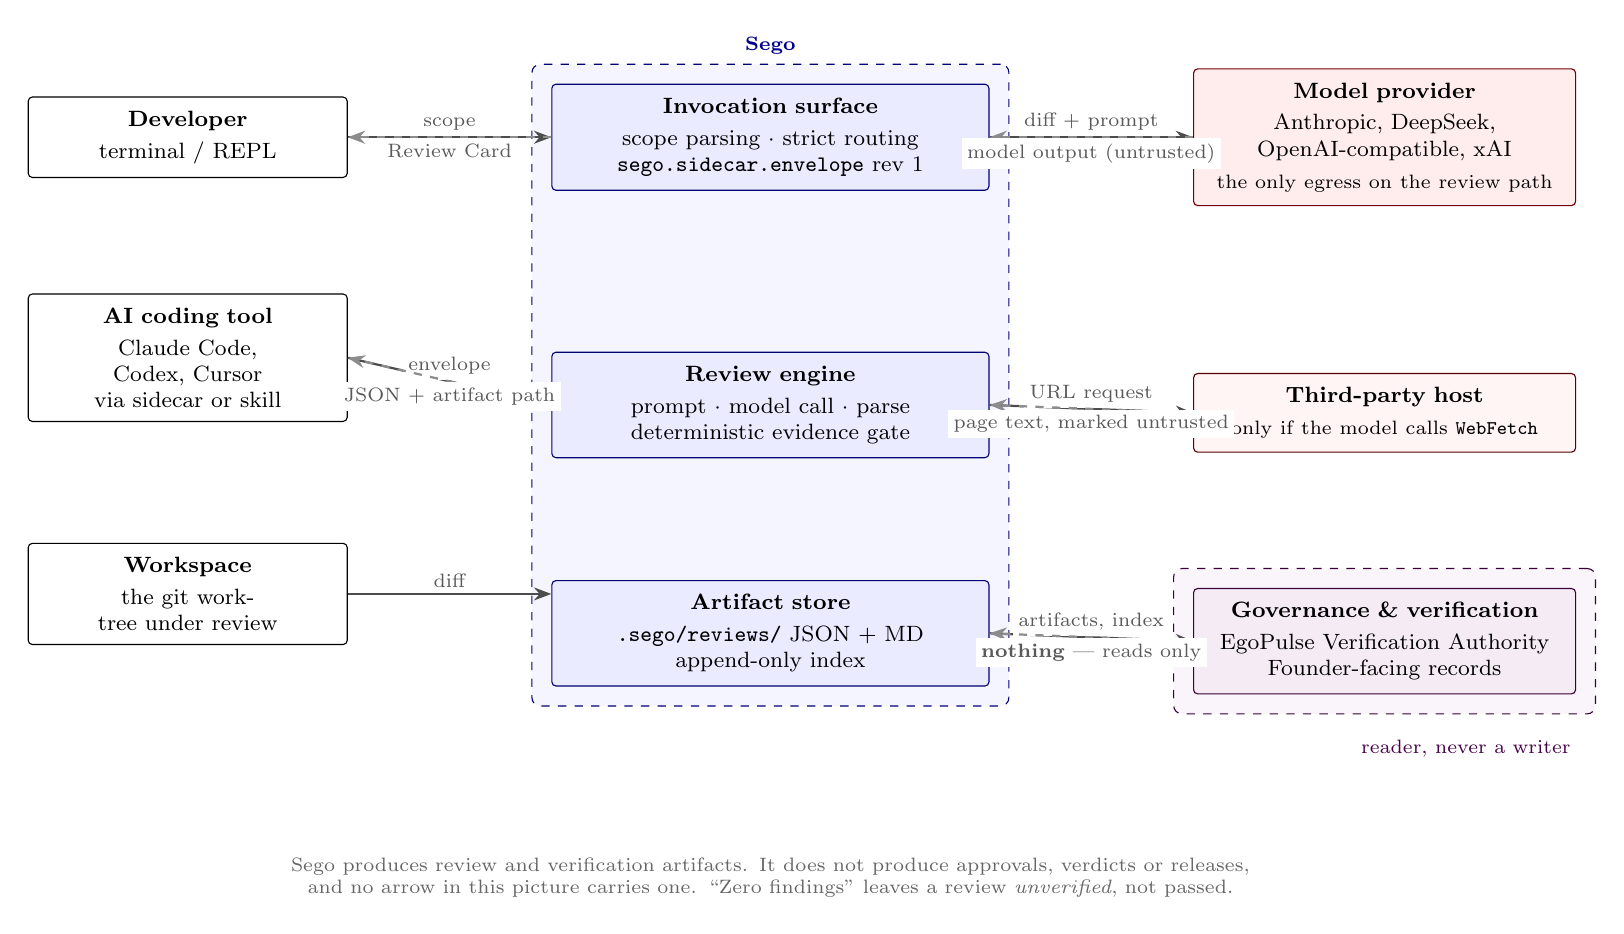
\begin{tikzpicture}[
  x=1cm, y=1cm,
  font=\small,
  box/.style={draw, rounded corners=1.5pt, fill=white, font=\footnotesize,
              align=center, inner sep=5pt},
  mine/.style={box, fill=blue!8, draw=blue!45!black},
  arr/.style={-{Stealth[length=2.2mm]}, thick, draw=black!70},
  ret/.style={-{Stealth[length=2.2mm]}, thick, draw=black!45, dashed},
  lab/.style={font=\scriptsize, text=black!65, inner sep=2pt, fill=white},
  grp/.style={draw=black!25, dashed, rounded corners=3pt, inner sep=7pt}
]

% ---------------- centre: three panels, one per traffic row ----------------
\node[mine, text width=52mm] (surf) at (0, 3.4)
  {\textbf{Invocation surface}\\[2pt] \footnotesize scope parsing $\cdot$ strict routing\\
   \footnotesize \texttt{sego.sidecar.envelope} rev 1};
\node[mine, text width=52mm] (eng) at (0, 0.0)
  {\textbf{Review engine}\\[2pt] \footnotesize prompt $\cdot$ model call $\cdot$ parse\\
   \footnotesize deterministic evidence gate};
\node[mine, text width=52mm] (store) at (0, -2.9)
  {\textbf{Artifact store}\\[2pt] \footnotesize \texttt{.sego/reviews/} JSON + MD\\
   \footnotesize append-only index};

\begin{scope}[on background layer]
  \node[grp, draw=blue!45!black, fill=blue!4,
        label={[font=\scriptsize\bfseries, text=blue!55!black]above:Sego}] (segobox)
    [fit=(surf)(eng)(store)] {};
\end{scope}

% ---------------- left: intent in ----------------
\node[box, text width=37mm] (dev) at (-7.4, 3.4)
  {\textbf{Developer}\\[2pt] \footnotesize terminal / REPL};
\node[box, text width=37mm] (agent) at (-7.4, 0.6)
  {\textbf{AI coding tool}\\[2pt] \footnotesize Claude Code, Codex, Cursor\\ \footnotesize via sidecar or skill};
\node[box, text width=37mm] (ws) at (-7.4, -2.4)
  {\textbf{Workspace}\\[2pt] \footnotesize the git worktree under review};

\draw[arr] (dev.east) -- node[lab, above] {scope} (surf.west);
\draw[ret] (surf.west) -- node[lab, below] {Review Card} (dev.east);
\draw[arr] (agent.east) -- node[lab, above] {envelope} (eng.west);
\draw[ret] (eng.west) -- node[lab, below] {JSON + artifact path} (agent.east);
\draw[arr] (ws.east) -- node[lab, above] {diff} (eng.west |- ws);

% ---------------- right: where data goes ----------------
\node[box, text width=45mm, fill=red!7, draw=red!45!black] (prov) at (7.8, 3.4)
  {\textbf{Model provider}\\[2pt] \footnotesize Anthropic, DeepSeek,\\ \footnotesize OpenAI-compatible, xAI\\[2pt]
   \scriptsize the only egress on the review path};
\node[box, text width=45mm, fill=red!4, draw=red!35!black] (web) at (7.8, -0.1)
  {\textbf{Third-party host}\\[2pt] \scriptsize only if the model calls \texttt{WebFetch}};
\node[box, text width=45mm, fill=violet!8, draw=violet!45!black] (gov) at (7.8, -3.0)
  {\textbf{Governance \& verification}\\[2pt] \footnotesize EgoPulse Verification Authority\\ \footnotesize Founder-facing records};

\draw[arr] (surf.east) -- node[lab, above] {diff + prompt} (prov.west);
\draw[ret] (prov.west) -- node[lab, below] {model output (untrusted)} (surf.east);
\draw[arr] (eng.east) -- node[lab, above] {URL request} (web.west);
\draw[ret] (web.west) -- node[lab, below] {page text, marked untrusted} (eng.east);
\draw[arr] (store.east) -- node[lab, above] {artifacts, index} (gov.west);
\draw[ret] (gov.west) -- node[lab, below] {\textbf{nothing} — reads only} (store.east);

\begin{scope}[on background layer]
  \node[grp, draw=violet!45!black, fill=violet!4] (govbox) [fit=(gov)] {};
\end{scope}
\node[font=\scriptsize, text=violet!55!black, anchor=north east]
  at ([xshift=-2mm, yshift=-2mm]govbox.south east) {reader, never a writer};

\node[font=\scriptsize, text=black!60, text width=180mm, align=center] at (0, -6.0)
  {Sego produces review and verification artifacts. It does not produce approvals, verdicts or releases, and no arrow in
   this picture carries one. ``Zero findings'' leaves a review \emph{unverified}, not passed.};

\end{tikzpicture}
\end{document}
